\documentclass[aspectratio=169,11pt]{beamer}

\usepackage[T1]{fontenc}
\usepackage{helvet}
\renewcommand{\familydefault}{\sfdefault}
\usepackage{graphicx}
\usepackage{tikz}
\usetikzlibrary{arrows.meta,calc,positioning}

\definecolor{titlebg}{HTML}{1B1B36}
\definecolor{accent}{HTML}{FF6846}
\definecolor{flowblue}{HTML}{6657FF}
\definecolor{portblue}{HTML}{174CFF}
\definecolor{boxfill}{HTML}{F7F7F7}
\definecolor{boxborder}{HTML}{555555}
\definecolor{nginxfill}{HTML}{F4C3A7}
\definecolor{muted}{HTML}{666666}

\setbeamertemplate{navigation symbols}{}
\setbeamertemplate{footline}{}
\setbeamertemplate{headline}{}
\setbeamersize{text margin left=0pt,text margin right=0pt}
\setbeamercolor{normal text}{fg=black,bg=white}
\setbeamerfont{normal text}{size=\normalsize}

% Logo helper: the deck still compiles before the PNGs are added.
\newcommand{\maybeimage}[3][]{%
  \IfFileExists{#2}{\includegraphics[#1]{#2}}{\textcolor{muted}{\scriptsize\textbf{#3}}}%
}

\tikzset{
  service/.style={
    draw=boxborder,
    fill=boxfill,
    line width=0.7pt,
    rounded corners=1pt,
    minimum width=2.72cm,
    minimum height=1.17cm,
    inner sep=3pt,
    align=center
  },
  nginxservice/.style={service,fill=nginxfill},
  flow/.style={-{Stealth[length=2.2mm,width=1.6mm]},draw=flowblue,line width=1.25pt},
  monitor/.style={flow,dashed},
  flowlabel/.style={font=\scriptsize,text=black,fill=white,inner sep=1.4pt}
}

\begin{document}

% -----------------------------------------------------------------------------
% Title slide
% -----------------------------------------------------------------------------
{
\setbeamercolor{background canvas}{bg=titlebg}
\begin{frame}[plain,t]
\nointerlineskip
\begin{tikzpicture}[x=1mm,y=1mm]
  \useasboundingbox (0,0) rectangle (160,90);

  \node[anchor=west,text=white,font=\bfseries\fontsize{37}{40}\selectfont]
    at (8,80) {Project Defence};

  \node[anchor=west,text=accent,font=\bfseries\fontsize{36}{39}\selectfont]
    at (8,61) {Job Market};

  \node[anchor=west,fill=accent,text=white,inner xsep=1.5mm,inner ysep=0.8mm,
        font=\fontsize{18}{20}\selectfont]
    at (8,36) {DATA OPS};

  \node[anchor=west,text=white,font=\fontsize{16}{18}\selectfont]
    at (12,7) {Sergey Krutikov};
\end{tikzpicture}
\end{frame}
}

% -----------------------------------------------------------------------------
% Architecture slide
%
% Overlay order:
%  1 Browser
%  2 Nginx
%  3 frontend
%  4 backend
%  5 PostgreSQL
%  6 Elasticsearch
%  7 Airflow
%  8 Prometheus
%  9 Grafana
% 10 Pushgateway
% 11 Alertmanager
%
% Each arrow appears on the first overlay on which both of its endpoint
% nodes exist. This implements the requested predecessor/successor rule.
% -----------------------------------------------------------------------------
\begin{frame}[plain,t]
\nointerlineskip
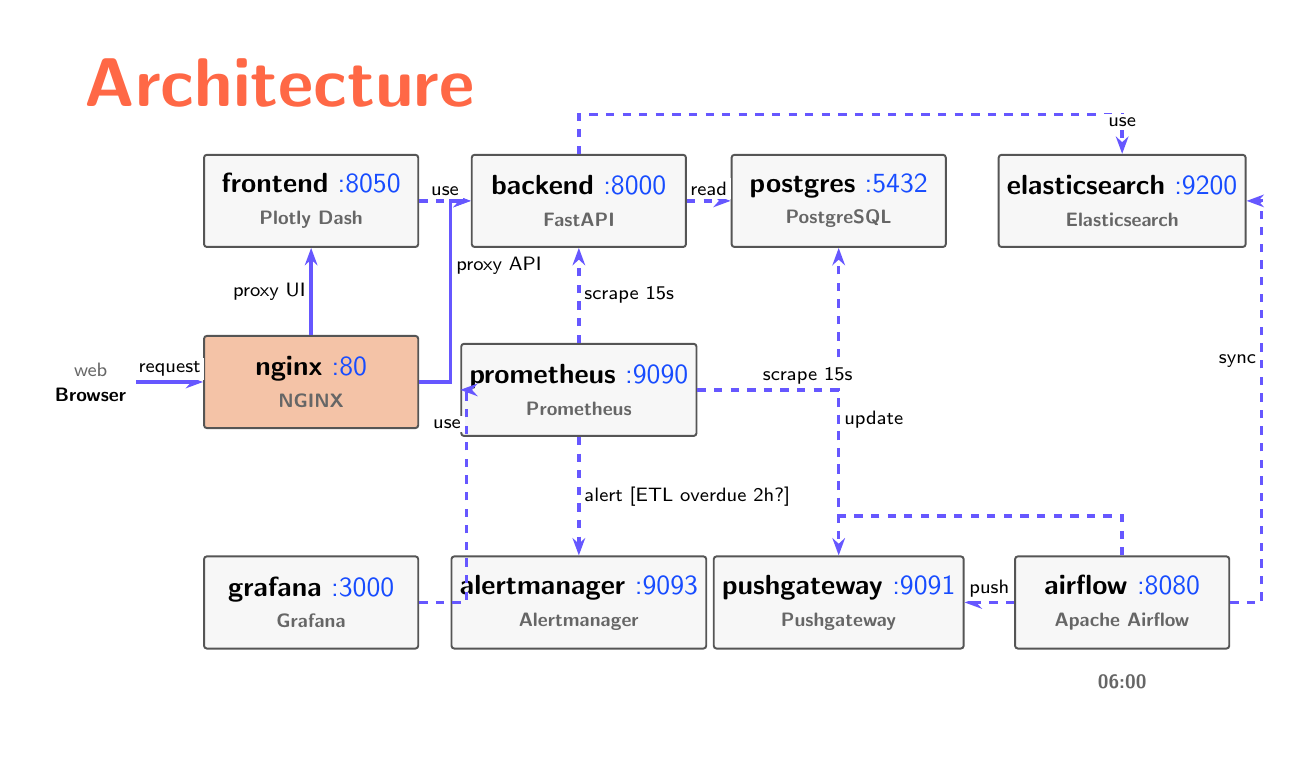
\begin{tikzpicture}[x=1mm,y=1mm]
  \useasboundingbox (0,0) rectangle (160,90);

  \node[anchor=west,text=accent,font=\bfseries\fontsize{25}{28}\selectfont]
    at (6,83) {Architecture};

  % Overall topology follows docs/images/docker-deployment.png.
  \coordinate (browserpos) at (8,45);
  \coordinate (nginxpos) at (36,45);
  \coordinate (frontendpos) at (36,68);
  \coordinate (backendpos) at (70,68);
  \coordinate (postgrespos) at (103,68);
  \coordinate (elasticpos) at (139,68);
  \coordinate (prometheuspos) at (70,44);
  \coordinate (grafanapos) at (36,17);
  \coordinate (alertmanagerpos) at (70,17);
  \coordinate (pushgatewaypos) at (103,17);
  \coordinate (airflowpos) at (139,17);

  % Nodes ---------------------------------------------------------------------
  \node<1->[align=center] (browser) at (browserpos) {%
    \IfFileExists{../images/icons/browser.png}
      {\includegraphics[width=10mm]{../images/icons/browser.png}}
      {\textcolor{muted}{\scriptsize web}}\\[-1mm]
    \scriptsize\textbf{Browser}%
  };

  \node<2->[nginxservice] (nginx) at (nginxpos) {%
    \textbf{nginx} \textcolor{portblue}{:80}\\[-0.2mm]
    \maybeimage[height=5.4mm]{../images/logos/nginx.png}{NGINX}%
  };

  \node<3->[service] (frontend) at (frontendpos) {%
    \textbf{frontend} \textcolor{portblue}{:8050}\\[-0.2mm]
    \maybeimage[height=5.2mm]{../images/logos/dash.png}{Plotly Dash}%
  };

  \node<4->[service] (backend) at (backendpos) {%
    \textbf{backend} \textcolor{portblue}{:8000}\\[-0.2mm]
    \maybeimage[height=5.2mm]{../images/logos/fastapi.png}{FastAPI}%
  };

  \node<5->[service] (postgres) at (postgrespos) {%
    \textbf{postgres} \textcolor{portblue}{:5432}\\[-0.2mm]
    \maybeimage[height=5.5mm]{../images/logos/postgres.png}{PostgreSQL}%
  };

  \node<6->[service] (elasticsearch) at (elasticpos) {%
    \textbf{elasticsearch} \textcolor{portblue}{:9200}\\[-0.2mm]
    \maybeimage[height=5.5mm]{../images/logos/elasticsearch.png}{Elasticsearch}%
  };

  \node<7->[service] (airflow) at (airflowpos) {%
    \textbf{airflow} \textcolor{portblue}{:8080}\\[-0.2mm]
    \maybeimage[height=5.4mm]{../images/logos/airflow.png}{Apache Airflow}%
  };
  \node<7->[anchor=north,font=\scriptsize,text=portblue]
    at ([yshift=-2mm]airflow.south) {%
      \maybeimage[width=10mm]{../images/icons/06-00.png}{06:00}%
    };

  \node<8->[service] (prometheus) at (prometheuspos) {%
    \textbf{prometheus} \textcolor{portblue}{:9090}\\[-0.2mm]
    \maybeimage[height=5.4mm]{../images/logos/prometheus.png}{Prometheus}%
  };

  \node<9->[service] (grafana) at (grafanapos) {%
    \textbf{grafana} \textcolor{portblue}{:3000}\\[-0.2mm]
    \maybeimage[height=5.4mm]{../images/logos/grafana.png}{Grafana}%
  };

  % Pushgateway and Alertmanager use the Prometheus family logo in the source
  % diagram, so the Prometheus image is reused for them here.
  \node<10->[service] (pushgateway) at (pushgatewaypos) {%
    \textbf{pushgateway} \textcolor{portblue}{:9091}\\[-0.2mm]
    \maybeimage[height=5.0mm]{../images/logos/prometheus.png}{Pushgateway}%
  };

  \node<11->[service] (alertmanager) at (alertmanagerpos) {%
    \textbf{alertmanager} \textcolor{portblue}{:9093}\\[-0.2mm]
    \maybeimage[height=5.0mm]{../images/logos/prometheus.png}{Alertmanager}%
  };

  % Arrows --------------------------------------------------------------------
  % Browser -> Nginx
  \draw<2->[flow]
    (browser.east) -- node[flowlabel,above]{request} (nginx.west);

  % Nginx -> frontend
  \draw<3->[flow]
    (nginx.north) -- node[flowlabel,left]{proxy UI} (frontend.south);

  % Nginx -> backend and frontend -> backend
  \draw<4->[flow]
    (nginx.east) -- ++(4mm,0) |- node[flowlabel,pos=0.32,right]{proxy API} (backend.west);
  \draw<4->[monitor]
    (frontend.east) -- node[flowlabel,above]{use} (backend.west);

  % backend -> PostgreSQL
  \draw<5->[monitor]
    (backend.east) -- node[flowlabel,above]{read} (postgres.west);

  % backend -> Elasticsearch
  \draw<6->[monitor]
    (backend.north) -- ++(0,5mm) -|
    node[flowlabel,pos=0.72,above]{use} (elasticsearch.north);

  % Airflow -> PostgreSQL and Elasticsearch
  \draw<7->[monitor]
    (airflow.north) -- ++(0,5mm) -|
    node[flowlabel,pos=0.68,right]{update} (postgres.south);
  \draw<7->[monitor]
    (airflow.east) -- ++(4mm,0) |-
    node[flowlabel,pos=0.30,left]{sync} (elasticsearch.east);

  % Prometheus -> backend
  \draw<8->[monitor]
    (prometheus.north) --
    node[flowlabel,right]{scrape $\circlearrowleft$15s} (backend.south);

  % Grafana -> Prometheus
  \draw<9->[monitor]
    (grafana.east) -- ++(6mm,0) |-
    node[flowlabel,pos=0.42,left]{use} (prometheus.west);

  % Airflow -> Pushgateway; Prometheus -> Pushgateway
  \draw<10->[monitor]
    (airflow.west) -- node[flowlabel,above]{push} (pushgateway.east);
  \draw<10->[monitor]
    (prometheus.east) -- ++(9mm,0) -|
    node[flowlabel,pos=0.28,above]{scrape $\circlearrowleft$15s} (pushgateway.north);

  % Prometheus -> Alertmanager
  \draw<11->[monitor]
    (prometheus.south) --
    node[flowlabel,right]{alert [ETL overdue 2h?]} (alertmanager.north);

\end{tikzpicture}
\end{frame}

\end{document}
